\section{File \texttt{N.vtu}}

\begin{figure}[H]
    \centering
    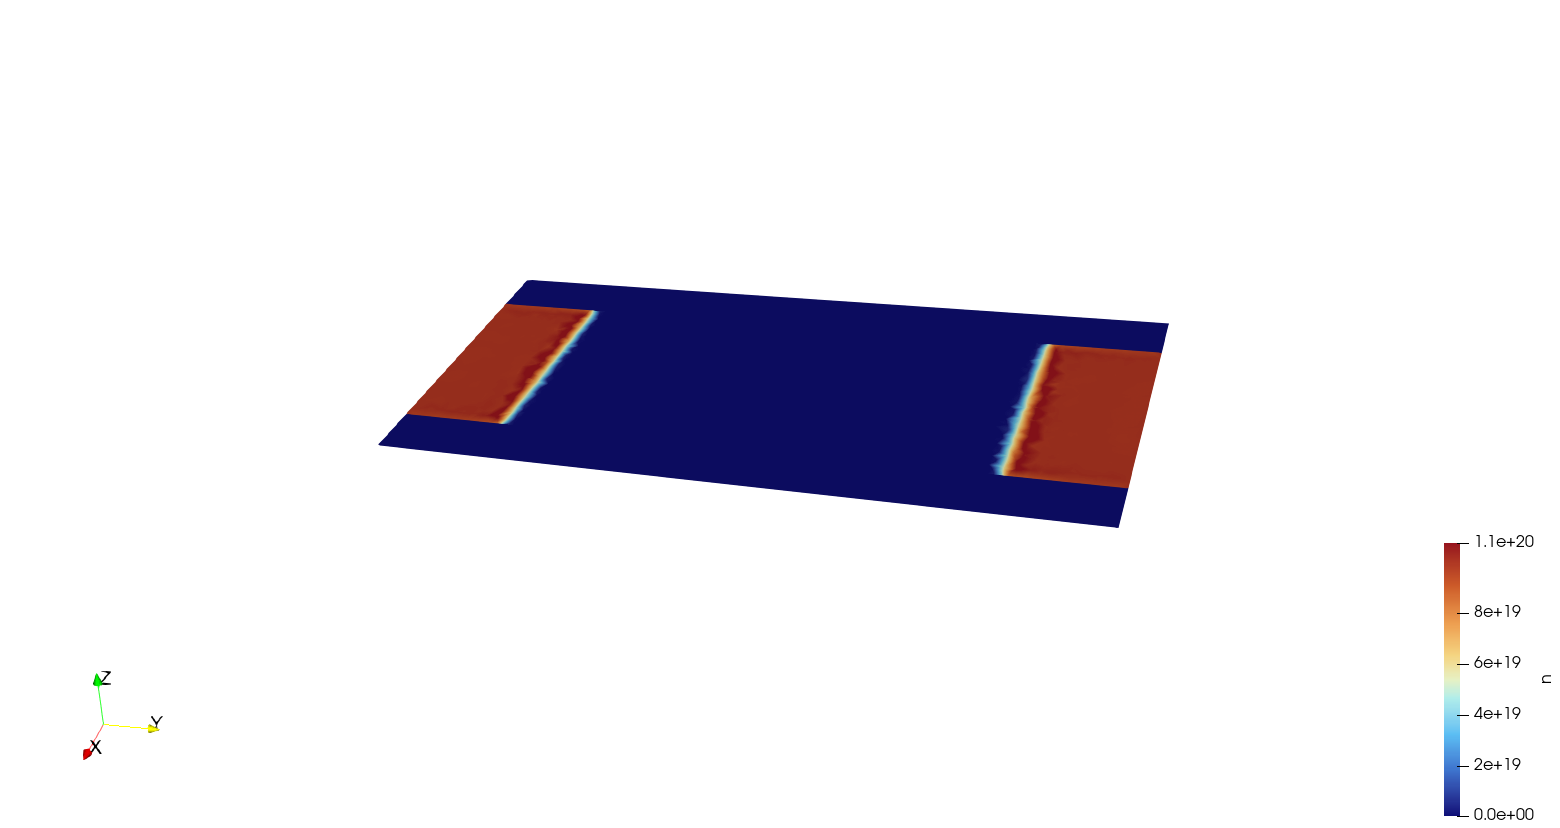
\includegraphics[width=0.7\textwidth, trim=0 0 0 170, clip]{Davide/Prova.png}
    \caption{Electron density \(n\) on the central slice of the device.}
    \label{fig:n-file-paraview}
\end{figure}

Figure~\ref{fig:n-file-paraview} shows that the electron density is concentrated in the source and drain regions, while it is almost zero in the central region where the dots are located. This is consistent with the electrostatic potential obtained from the Poisson solver: the gates create high barriers between the reservoirs and the dots, raising the local conduction-band energy and depleting the dot region. Therefore, at this stage of the simulation the carriers remain mainly in the doped contacts rather than populating the quantum dots.
